\section{Security in the pipeline}
Security in the pipeline is the process of implementing different measures and controls to protect the code that is being sent through the pipeline from various security threats. The pipeline commonly consists of multiple phases like code development, testing, and deployment, all of which may be susceptible to various security threats, like unauthorized access, data breaches, malware, and denial-of-service attacks. Security in the pipeline is crucial to secure the integrity and confidentiality of software applications and data.

\subsection{Code Scanning}
%du tester koden som skal bli deployet, alstå det som ligger inni pipelinen. Sjekkes for sårbarheter etc
Code scanning is a security measure where code is analyzed with the help of a tool to find security vulnerabilities and coding errors. Code scanning serves as a preventive measure against developers introducing new issues. During this step, you can perform a SAST scan using specialized tools that are designed to scan through code. 
\\
\\
GitHub provides an integrated code scanner called CodeQL. CodeQL extracts all source code into a relational database optimized for CodeQL analysis.  It can then be queried to identify insecure patterns in the code and other vulnerabilities. The user can take advantage of a large number of queries already made by other developers, or they can make their own. An example of a simple query could be getting the location of all method calls in the code. 
 \cite{codeql}

 \vspace{2mm}
\begin{figure}[H]
    \centering
    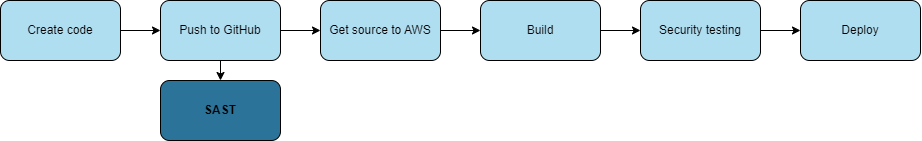
\includegraphics[width=0.8\columnwidth]{Images/pipeline2.png}
    \caption{Pipeline with implemented SAST scan}
    \label{fig: Pipeline with implemented SAST scan}
\end{figure}

\subsection{Scan Dependencies and Open Source Libraries}
All dependencies, open-source libraries, and third-party \gls{artifact}s that have been utilized should be validated. This can be done by comparing their checksum against a reliable, good source and validating any cryptographic signatures. If any third-party software was implemented in the application it's important to conduct an \acrshort{sca} scan using suitable tools to identify whether any vulnerable open-source software was used. \cite{bestpracticeSupplyChain}

\vspace{2mm}
\begin{figure}[H]
    \centering
    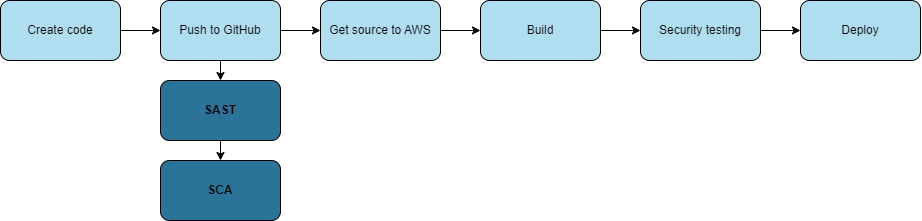
\includegraphics[width=0.8\columnwidth]{Images/pipeline3.png}
    \caption{Pipeline with implemented SCA scan}
    \label{fig: Pipeline with implemented SCA scan}
\end{figure}

\subsection{Secret Scanning}
To prevent or identify accidental exposure of "secrets", like access tokens, SSH keys, or other credentials, one should execute a secret scanning on a Git repository. Secret scanning tools, such as GitHub's secret scanning, can be used to find these vulnerabilities, and alert developers to potential security risks. \cite{GithubSecretScanning}

\vspace{2mm}
\begin{figure}[H]
    \centering
    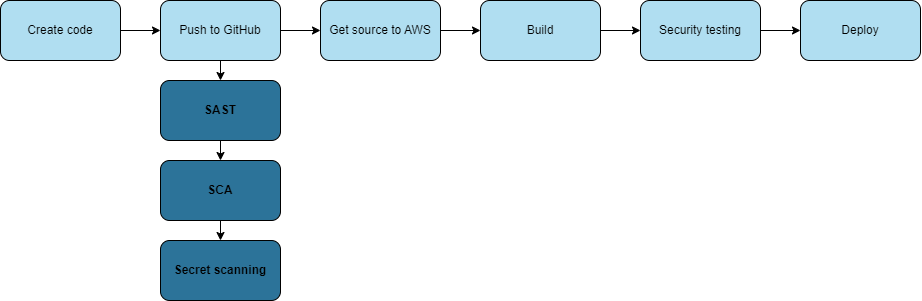
\includegraphics[width=0.8\columnwidth]{Images/pipeline4.png}
    \caption{Pipeline with implemented secret scan}
    \label{fig: Pipeline with implemented secret scan}
\end{figure}

\subsection{Dynamic scanning}
In software best practices, it is recommended to run multiple tests and scans to identify bugs and errors - where one of these tests is \acrlong{dast} (\acrshort{dast}).\cite{bestpracticeSupplyChain} This scanning method tries to penetrate the application, attempting to identify vulnerabilities and weaknesses in it. One can implement a tool specialized for DAST scans, such as OWASP Zap, which can identify security risks like \gls{Cross-site scripting}, \gls{SQL-injection} or path traversal.\cite{dynamictesting}


\subsubsection{The Limitations of DAST Tools}
Even though \acrshort{dast} can be used to identify potential vulnerabilities, certain types of threats may go undetected. For this reason, the company should engage a red team, which is a group of experts capable of performing penetration testing. A pen test will provide a more realistic test, as it simulates a real-world attack, detects more complex vulnerabilities, and provide a more comprehensive view of an application's security posture. A pen test can also function as a validation of the \acrshort{dast} scan, as it can help determine if the vulnerability can be exploited and the potential impact of the vulnerability. \cite{dastpentesting}

\vspace{2mm}
\begin{figure}[H]
    \centering
    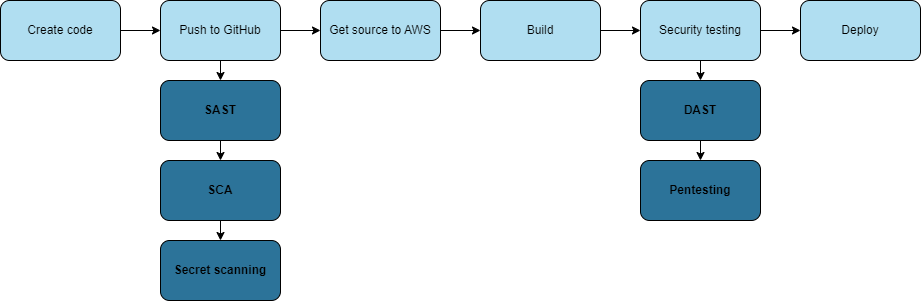
\includegraphics[width=0.8\columnwidth]{Images/pipeline5.png}
    \caption{Pipeline with implemented DAST scan and pentesting}
    \label{fig: Pipeline with implemented DAST scan and pentesting}
\end{figure}

\subsection{Artifacts}



